% Lecture notes: Week 9, Lecture 2 -- Stress Concentrations
% To hide this lecture from the website, add a line containing only:  % draft
% To set the date shown on the website, add a line like:  % posted: 2026-09-02
% Uses the image figures/w09l2_fe_plate_hole.png (path relative to the repository root).
\documentclass[11pt]{article}
\usepackage{mech2030notes}
\begin{document}

% ##################################################################
%  WEEK 9, LECTURE 2
% ##################################################################
\lecture{9}{2}{Stress Concentrations}

\noindent
$\rightarrow$ How do the stresses in an axially loaded plate change if a \emph{hole} is
drilled in the center? What if \emph{fillets} are present?

% ------------------------------------------------------------------
% Three plates (top row) and the stress on a cut through each (bottom row)
% ------------------------------------------------------------------
\begin{center}
\begin{minipage}[t]{0.31\textwidth}
\centering
\textbf{Axially loaded plate}\\[0.5em]
\begin{tikzpicture}
  \draw[thick, fill=gray!12] (-0.7,-1) rectangle (0.7,1);
  \draw[force] (0,1.02) -- (0,1.7) node[right] {$P$};
  \draw[force] (0,-1.02) -- (0,-1.7) node[right] {$P$};
\end{tikzpicture}

\vspace{0.8em}
\begin{tikzpicture}
  \draw[thick, fill=gray!12] (-0.7,-1) rectangle (0.7,0);
  \foreach \x in {-0.7,-0.525,...,0.71}
    \draw[-{Stealth[length=1.5mm,width=1.1mm]}, semithick] (\x,0) -- (\x,0.5);
  \draw[plotline] (-0.7,0.5) -- (0.7,0.5);
  \node[above] at (0,0.5) {$\sigma_{\text{avg}}$};
  \draw[force] (0,-1.02) -- (0,-1.7) node[right] {$P$};
\end{tikzpicture}
\end{minipage}%
\hfill
\begin{minipage}[t]{0.31\textwidth}
\centering
\textbf{Plate with a hole}\\[0.5em]
\begin{tikzpicture}
  \draw[thick, fill=gray!12] (-0.7,-1) rectangle (0.7,1);
  \draw[thick, fill=white] (0,0) circle (0.15);
  \draw[force] (0,1.02) -- (0,1.7) node[right] {$P$};
  \draw[force] (0,-1.02) -- (0,-1.7) node[right] {$P$};
\end{tikzpicture}

\vspace{0.8em}
\begin{tikzpicture}
  % lower half, cut through the hole; stress along the cut from the Kirsch solution:
  % sigma/sigma_inf = 1 + r^2/(2x^2) + 3r^4/(2x^4)   (r = 0.15, sigma_inf -> 0.45 cm)
  \fill[gray!12] (-0.7,-1) rectangle (0.7,0);
  \fill[white] (0.15,0) arc (0:-180:0.15) -- cycle;
  \draw[thick] (-0.7,0) -- (-0.7,-1) -- (0.7,-1) -- (0.7,0) -- (0.15,0)
               arc (0:-180:0.15) -- cycle;
  \foreach \x in {0.15,0.22,0.31,0.42,0.55,0.7} {
    \pgfmathsetmacro{\s}{0.45*(1 + 0.15^2/(2*\x^2) + 3*0.15^4/(2*\x^4))}
    \draw[-{Stealth[length=1.5mm,width=1.1mm]}, semithick] (\x,0) -- (\x,\s);
    \draw[-{Stealth[length=1.5mm,width=1.1mm]}, semithick] (-\x,0) -- (-\x,\s);
  }
  \draw[plotline] plot[domain=0.15:0.7, samples=30]
        (\x,{0.45*(1 + 0.15^2/(2*\x^2) + 3*0.15^4/(2*\x^4))});
  \draw[plotline] plot[domain=0.15:0.7, samples=30]
        (-\x,{0.45*(1 + 0.15^2/(2*\x^2) + 3*0.15^4/(2*\x^4))});
  \node[above] at (0,1.4) {$\sigma_{\max}$};
  \node[left] at (-0.72,0.55) {$\sigma_{\text{avg}}$};
  \draw[force] (0,-1.02) -- (0,-1.7) node[right] {$P$};
\end{tikzpicture}
\end{minipage}%
\hfill
\begin{minipage}[t]{0.31\textwidth}
\centering
\textbf{Plate with fillets}\\[0.5em]
\begin{tikzpicture}
  \draw[thick, fill=gray!12]
    (-0.7,1) -- (0.7,1) -- (0.7,0.7) arc (90:180:0.25) -- (0.45,-0.45)
    arc (180:270:0.25) -- (0.7,-1) -- (-0.7,-1) -- (-0.7,-0.7)
    arc (-90:0:0.25) -- (-0.45,0.45) arc (0:90:0.25) -- cycle;
  \draw[force] (0,1.02) -- (0,1.7) node[right] {$P$};
  \draw[force] (0,-1.02) -- (0,-1.7) node[right] {$P$};
\end{tikzpicture}

\vspace{0.8em}
\begin{tikzpicture}
  % lower part, cut at the base of the fillets (schematic distribution)
  \draw[thick, fill=gray!12]
    (-0.45,0) -- (0.45,0) arc (180:270:0.25) -- (0.7,-0.6) -- (-0.7,-0.6)
    -- (-0.7,-0.25) arc (-90:0:0.25) -- cycle;
  \foreach \x in {0,0.15,0.27,0.36,0.45} {
    \pgfmathsetmacro{\s}{0.55 + 0.75*(\x/0.45)^4}
    \draw[-{Stealth[length=1.5mm,width=1.1mm]}, semithick] (\x,0) -- (\x,\s);
    \draw[-{Stealth[length=1.5mm,width=1.1mm]}, semithick] (-\x,0) -- (-\x,\s);
  }
  \draw[plotline] plot[domain=-0.45:0.45, samples=30] (\x,{0.55 + 0.75*(\x/0.45)^4});
  \node[above] at (0.45,1.3) {$\sigma_{\max}$};
  \node[left] at (-0.72,0.45) {$\sigma_{\text{avg}}$};
  \draw[force] (0,-0.62) -- (0,-1.3) node[right] {$P$};
\end{tikzpicture}
\end{minipage}
\end{center}

\begin{itemize}[label=$\rightarrow$]
  \item These features produce \emph{stress concentrations}, where the stress is often
        2--5$\times$ higher near the hole or fillet.
  \item The maximum stress is characterized by the \emph{stress concentration factor} (SCF):
        \[ \boxed{K = \frac{\sigma_{\max}}{\sigma_{\text{avg}}}} \]
\end{itemize}

% ==================================================================
\section*{How Do We Determine $K$?}
% ==================================================================

\noindent
There are three methods:
\begin{enumerate}
  \item \textbf{Analytical solutions} exist for some specific cases, but for most geometries
        analytical solutions are not possible.
  \item \textbf{Experimental techniques} such as photoelasticity or strain gauges can be used
        to measure the local stress.
        (Video demonstration of both:
        \href{https://youtu.be/pP9tcpDLOPI?t=220}{\texttt{youtu.be/pP9tcpDLOPI}}.)
  \item \textbf{Computational techniques} such as the finite-element method can solve for
        the full distribution of stresses, from which we can extract $\sigma_{\max}$.
\end{enumerate}
\begin{itemize}[label=\then]
  \item These days, (3) is the most common approach.
\end{itemize}

\begin{center}
  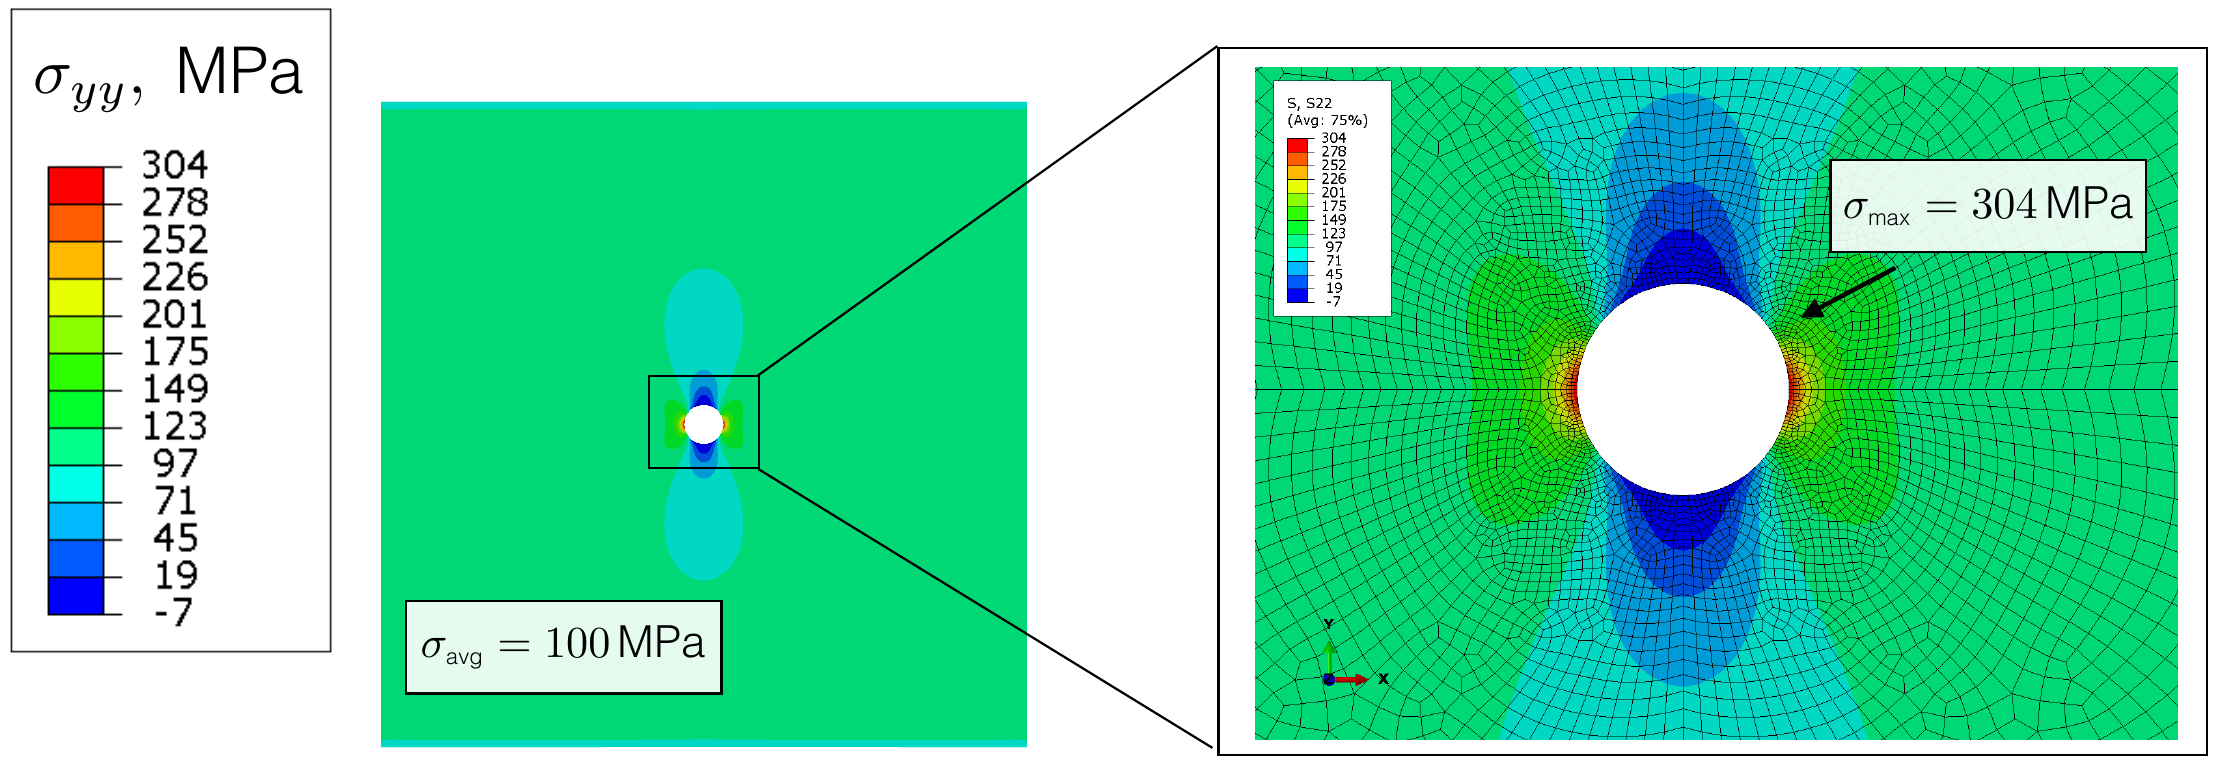
\includegraphics[width=\textwidth]{figures/w09l2_fe_plate_hole.png}\\[0.4em]
  \parbox{0.92\textwidth}{\small\centering
  Elastic finite-element analysis (Abaqus) of a plate with a small hole under uniaxial
  tension. The stress $\sigma_{yy}$ peaks at the edges of the hole:
  $\sigma_{\max}/\sigma_{\text{avg}} = 304/100 = 3.04$,
  a numerical stress concentration factor.}
\end{center}

% ==================================================================
\section*{Reference Curves}
% ==================================================================

\noindent
Using these techniques, we can collect SCFs for many different geometries and make
reference curves. For these curves, the average stress is computed on the
\emph{net} (smallest) cross-section:
\[
  \boxed{\sigma_{\text{avg}} = \frac{P}{t\,d}}
\]

\begin{center}
\begin{tikzpicture}
  % axes: 2r/D from 0 to 0.7 (10 cm per unit), K from 1.0 to 3.4 (2 cm per unit)
  \begin{scope}[x=10cm, y=2cm]
    \foreach \x in {0,0.1,...,0.71} \draw[gray!40, thin] (\x,1) -- (\x,3.4);
    \foreach \y in {1,1.2,...,3.41} \draw[gray!40, thin] (0,\y) -- (0.7,\y);
    \draw[semithick] (0,1) rectangle (0.7,3.4);
    \foreach \x in {0,0.1,...,0.71}
      \node[below, font=\small] at (\x,1) {\pgfmathprintnumber[fixed, precision=1]{\x}};
    \foreach \y in {1,1.4,...,3.41}
      \node[left, font=\small] at (0,\y) {\pgfmathprintnumber[fixed, precision=1, fixed zerofill]{\y}};
    \node[below=14pt] at (0.35,1) {$2r/D$};
    \node[left=18pt] at (0,2.2) {$K$};
    \draw[very thick, red!70!black] plot[domain=0:0.7, samples=60]
          (\x,{3 - 3.14*\x + 3.667*\x^2 - 1.527*\x^3});
    % worked-example marker
    \draw[densely dashed, thin] (0.4,1) -- (0.4,2.233) -- (0,2.233);
    \node[pin] at (0.4,2.233) {};
  \end{scope}
  % inset sketch: flat bar with a hole
  \fill[white] (2.75,5.25) rectangle (6.95,6.75);
  \begin{scope}[shift={(3.75,6.0)}]
    \draw[thick, fill=gray!12] (0,-0.55) rectangle (2.2,0.55);
    \draw[thick, fill=white] (1.1,0) circle (0.2);
    \draw[thin] (1.1,0) -- (1.24,0.14); \node[font=\scriptsize, above right] at (1.2,0.1) {$r$};
    \draw[{Stealth[length=1.5mm]}-{Stealth[length=1.5mm]}, thin] (1.8,-0.55) -- (1.8,0.55) node[midway, right, font=\small] {$D$};
    \draw[{Stealth[length=1.5mm]}-{Stealth[length=1.5mm]}, thin] (0.75,0.2) -- (0.75,0.55);
    \node[left, font=\scriptsize] at (0.75,0.38) {$\tfrac12 d$};
    \draw[{Stealth[length=1.5mm]}-{Stealth[length=1.5mm]}, thin] (0.75,-0.2) -- (0.75,-0.55);
    \node[left, font=\scriptsize] at (0.75,-0.38) {$\tfrac12 d$};
    \draw[force] (-0.05,0) -- (-0.6,0) node[left] {$P$};
    \draw[force] (2.25,0) -- (2.8,0) node[right] {$P$};
  \end{scope}
\end{tikzpicture}\\[0.4em]
\parbox{0.92\textwidth}{\small\centering
  SCF for a flat bar with a central hole, with $d = D - 2r$.
  Curve: $K = 3.000 - 3.140\,(2r/D) + 3.667\,(2r/D)^2 - 1.527\,(2r/D)^3$, the standard fit
  from \emph{Peterson's Stress Concentration Factors}, which agrees with the chart in
  Beer et al.\ (2012) to within a few percent.}
\end{center}

\noindent
For flat bars with \emph{fillets} ($K$ versus $r/d$ for several values of $D/d$), see the
chart in Beer et al.\ (2012), also reproduced in the W9L2 slides.

% ==================================================================
\section*{Example Problem}
% ==================================================================

\noindent
\begin{minipage}[c]{0.62\textwidth}
\centering
\begin{tikzpicture}[scale=0.9, every node/.style={scale=0.95}]
  % front view (scale: 0.8 cm per inch)
  \draw[thick, fill=gray!12] (0,-1) rectangle (4,1);
  \draw[thick, fill=white] (2,0) circle (0.4);
  \draw[force] (-0.05,0) -- (-1.2,0) node[left] {$\SI{3350}{lb}$};
  \draw[force] (4.85,0) -- (6.0,0) node[right] {$\SI{3350}{lb}$};
  \draw[dim] (3.2,-1) -- (3.2,1) node[midway, right] {$2.5''$};
  \draw[thin] (1.6,-0.05) -- (1.6,-1.45) (2.4,-0.05) -- (2.4,-1.45);
  \draw[dim] (1.6,-1.35) -- (2.4,-1.35) node[midway, below] {$1''$};
  % side view showing the thickness t
  \draw[thick, fill=gray!12] (4.3,-1) rectangle (4.55,1);
  \draw[dim] (4.3,-1.35) -- (4.55,-1.35) node[midway, below] {$t$};
\end{tikzpicture}
\end{minipage}%
\hfill
\begin{minipage}[c]{0.35\textwidth}
\textbf{Q:} If $\sigma_{\text{allow}} = \SI{22}{ksi}$, what is the required
thickness $t$?
\end{minipage}

\bigskip
\begin{itemize}
  \item Average stress on the net section:
        \[
          \sigma_{\text{avg}} = \frac{P}{t\,d} = \frac{\SI{3350}{lb}}{(t)(2.5'' - 1'')}
          = \left(\frac{2233.33}{t}\right)\ \si{psi}
          \qquad (t \text{ in inches})
        \]
  \item Stress concentration factor:
        \[
          \frac{2r}{D} = \frac{1''}{2.5''} = 0.4
          \quad\longrightarrow\quad
          \boxed{K = 2.25} \quad \text{(from the curve)}
        \]
  \item Set the maximum stress equal to the allowable stress:
        \[
          \sigma_{\max} = K\,\sigma_{\text{avg}} = \sigma_{\text{allow}}
        \]
        \[
          \hookrightarrow\quad (2.25)\left(\frac{2233.33}{t}\right)\ \si{psi}
          = \SI{22e3}{psi}
        \]
        \[
          t = \left(\frac{2233.33}{\num{22e3}}\right)(2.25)
          \qquad\Rightarrow\qquad
          \fbox{\fbox{$t = 0.228''$}}
        \]
\end{itemize}

\end{document}
